In the Earth's mantle major solid state phase transitions occur in the 
silicate material which constitutes the planetary mantle
outside the metallic iron/nickle core.
These phase transitions are induced by the increase in the static
pressure from a 1 bar ($10^5$ Pa) atmospheric value at the Earth's surface to 
$136 \cdot 10^9 \mathrm{Pa}$ at the core mantle boundary at a depth of
approximately 2900 km.
Phase transitions in the Earth's interior are associated with changes 
in the elastic wave velocities that can be deduced from seismological 
observations.
In high pressure experiments, phase transitions in candidate mantle
silicates can be studied and correlated with the seismological data
to constrain the mineralogy and pressure/temperature distribution 
in the mantle.
Knowledge of the internal material constitution of the Earth,
such as the mineral phase,
is a requirement for understanding the main geodynamical processes that determine
Earth's evolution.

Density and pressure inside the Earth are linked with self-gravitation.
This means that the hydrostatic or lithostatic pressure is a direct 
result of the gravity field generated by the Earth's own mass 
distribution.
The lithostatic pressure can be expressed as the weight of a column
of unit cross-sectional area extending from zero depth, at the Earth's 
surface, to the depth $z$ of the evaluation point,
\begin{equation}
 P(z) = \int_0^z \rho(z') g(z') dz'
\label{def_pressure_integ}
\end{equation}
where $\rho$ is the mass density and $g$ is the magnitude of
the gravitational acceleration.

The gravity field defining $g$ is generated by the Earth's own density 
distribution.
Weak periodic gravity `perturbations' are generated by celestial
bodies, expressed in the external tides, both ocean tides and solid
earth tides.
The main tides are generated by the Earth's moon and by the Sun.

In the following section expressions for the gravity field in terms
of the density distribution are given, based on Newton's law of
gravitation.

In the description of the density distribution we will first neglect 
the role of self-compression and consider a number of one-dimensional 
(1-D), spherically symmetric, parameterized density distributions.
Self-compression and compressibility are then treated in section 
\ref{Pressure_density}.
Self-compression and finite compressibility result in a 
continuous increase of density with pressure in agreement 
with several geophysical observations.  

\vspace{0.5cm}
\fbox{
\begin{minipage}{0.9\textwidth}
\begin{problem}
\label{problem-pressure}
 {\small \it
  Derive the expression (\ref{def_pressure_integ}) 
  (where the depth $z$ is not to be confused with a 
   cartesian coordinate)
  for the lithostatic 
  pressure in a spherically
  symmetric planet from the elastostatic equation for a static medium,
  \begin{equation} 
     \partial_j \sigma_{ij} + \rho g_i = 0
  \label{elastostatic-eqn}
  \end{equation} 
  {\it Hint:}
  Assume hydrostatic conditions where the stress tensor 
  can be written as
  $\sigma_{ij}=-P\delta_{ij}$,
  with $\delta_{ij}$ the Kronecker delta,
  and derive from equation (\ref{elastostatic-eqn})
  for the pressure gradient, $\nabla P = \rho {\bf g}$. 
 }
\end{problem}
\end{minipage}
}

\vspace{0.5cm}

\subsubsection{Gravity field of a mass distribution}
Newton formulated the attraction force acting on a point 
mass $m_0$, 
located in a point with position vector ${\bf r}=(x,y,z)$,
with $x,y,z$ the cartesian coordinates,
from a second point mass $m_1$ located at
${\bf r}_1=(x_1,y_1,z_1)$, illustrated in the following figure as,
\begin{equation}
{\bf F} ({\bf r}) 
        =\frac{G m_0 m_1}{\left | {\bf r}_1 - {\bf r} \right | ^2} ~ 
          {\bf e}_{{\bf r r}_1}
\label{pointmass_gravity}
\end{equation}

\begin{center}
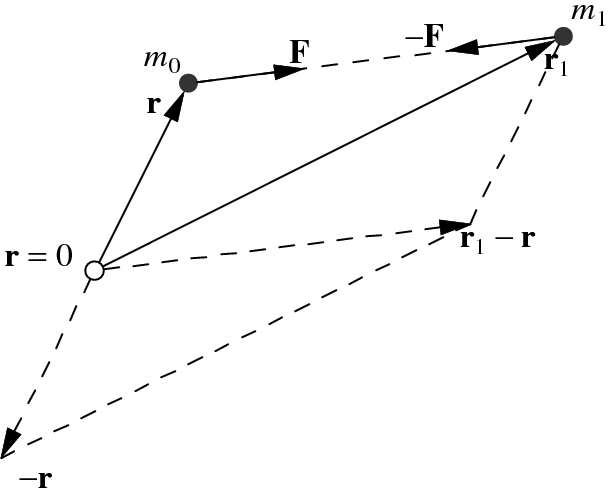
\includegraphics[width=7cm]{images/gravity/gravity_diagram.png}\\
{\captionfont Vector diagram of the gravitational forces acting on the two 
point masses $m_0$, $m_1$ in vector locations ${\bf r}$ and
${\bf r}_1$ respectively.
From the expression for the gravity field (\ref{pointmass_gravity}) 
it follows that the forces on both masses
are of equal magnitude and in opposite direction. }
\end{center}

Where ${\bf e}_{{\bf rr}_1}$ is the unit vector in 
${\bf r}$ pointing towards ${\bf r}_1$
and ${\bf F}({\bf r}_1) = - {\bf F}({\bf r})$.
${\bf r}, {\bf r}_1$ 
are the position vectors of the two point masses
and 
$\left | {\bf r}_1 - {\bf r} \right | =
\sqrt{(x_1-x)^2 + (y_1-y)^2 + (z_1-z)^2}$
is the distance between the points ${\bf r}$ and ${\bf r}_1$.
$G$ is the gravitational constant 
$G = 6.6732 \times 10^{-11} ~\mathrm{Nm^{2}kg^{-2}}$,
$m_0, m_1$ the mass of the respective pointmasses.




This gravitation effect is usually specified as a gravitation force per 
unit mass or acceleration vector ${\bf g}$,
\begin{equation}
{\bf g}({\bf r}) =
   \frac{G m_1}{\left | {\bf r}_1 - {\bf r} \right | ^2} ~ 
                {\bf e}_{{\bf r r}_1} 
\label{grav_accel}
\end{equation}
It can be verified by inspection that the acceleration vector field 
can be written as the 
gradient of a scalar potential field $U({\bf r})$ with
${\bf g} = - \nabla U = 
(- \frac{\partial U}{\partial x}, 
 - \frac{\partial U}{\partial y}, 
 - \frac{\partial U}{\partial z}
)$,
(see problem \ref{problem-verify-gradient}),
\begin{equation}
\boxed{U({\bf r}) = - \frac{G m_1}{\left | {\bf r}_1 - {\bf r} \right |} }
\label{grav_potential}
\end{equation}

The gravity acceleration and corresponding potential field are additive 
such that the total force or potential of a 
collection of $N$ point masses is obtained by summation over individual
point contributions,
\begin{equation}
{\bf g} ({\bf r}) = 
        \sum_j^N \frac{G m_j}{\left | {\bf r}_j - {\bf r} \right | ^2} ~ 
         {\bf e}_{{\bf r r}_j}
,\ \ 
U({\bf r}) = 
        - \sum_j^N \frac{G m_j}{\left | {\bf r}_j - {\bf r} \right |}
\end{equation}
With this definition and sign convention 
the potential field of
a point source in the origin is represented by a
potential well ($U({\bf r}) < 0$).
This is known as Coulomb's law and the equivalent form for a continuous
mass distribution of density $\rho$ (mass per unit volume) contained in
a volume $V$ is,
\begin{equation}
{\bf g}({\bf r}) = 
        \int_V \frac{G \rho({\bf r}^{'})}
                     {\left | {\bf r}^{'} - {\bf r} \right | ^2} ~ 
               {\bf e}_{{\bf r r}^{'}} ~ dV({\bf r}^{'})
,\ \ 
U({\bf r}) = 
        - \int_V \frac{G \rho({\bf r}^{'})}
                     {\left | {\bf r}^{'} - {\bf r} \right |} ~ 
               dV({\bf r}^{'})
\label{Coulomb-integrals}
\end{equation}

~\\
\noindent
Besides the integral expression for the gravity field defined in
(\ref{Coulomb-integrals}) there is also the differential form
using the second order partial differential equations of Laplace and
Poisson.
It can be shown by verification that $U$ in (\ref{Coulomb-integrals})
satisfies Poisson's equation, 
\begin{equation}
\boxed{\nabla^2 U = 4\pi G\rho}  \label{poisson_eqn}
\end{equation}
which reduces to Laplace's equation $\nabla^2 U = 0$
outside the mass distribution in $V$ (where $\rho =0$). 
\footnote{
To show that $U$ in (\ref{Coulomb-integrals}) satisfies Poisson's
equation integrate the normal component of the acceleration field
over an arbitrary closed surface $S$ enclosing $V$
and change the order of integration for the volume and surface
integral.
\begin{equation}
\int_S \nabla U({\bf r}) \cdot {\bf n} \ dA({\bf r})
   = - \int_V G \rho({\bf r}^{'}) 
    \left \{
     \int_S 
       \nabla 
       \left ( \frac{1}{\left | {\bf r}^{'}-{\bf r} \right |} \right )
      \cdot {\bf n} \ dA({\bf r}) 
    \right \} dV({\bf r}^{'})
\label{surface_integral}
\end{equation}
The surface integral on the right is independent of the choice of the
surface $S$ as long as it contains ${\bf r}^{'}$.
We therefore replace this surface by a sphere of radius $R$ centered
at $r^{'}$ and find for the surface integral the value $- 4 \pi$.
\newline
Next we apply the Gauss divergence theorem to the left hand surface 
integral to obtain,
\begin{equation}
\int_V \nabla^2 U \ dV = \int_V 4 \pi G \rho \ dV  
\label{int_form_poisson}
\end{equation}
Note that the surface has been contracted on the volume $V$
to obtain (\ref{int_form_poisson}).
Since the surface and enclosed volume are arbitrary we obtain the Poisson
equation,
\begin{equation}
\nabla^2 U  = 4 \pi G \rho 
\end{equation}
}

~\\
In Newton's time the numerical value of $G$ had not been
determined yet.
As a result it was not possible to determine the mass of the 
Earth $M_{\oplus}$ by measuring the gravitation force of the Earth 
on a known `test mass'.
This way only the value of $G M_{\oplus}$ could be determined.
Only with the experiment named after Cavendish (1798)
\footnote{
http://en.wikipedia.org/wiki/Cavendish\_experiment
}
it became possible
to measure $G$ directly, in a torsion balance experiment,
by determining the gravitational attraction of two closely spaced test 
masses.   

%----------------------------------------------------------------
%\subsubsection{Problem section: spherically symmetric density 
%distributions and corresponding gravity fields}



\vspace{0.5cm}
\fbox{
\begin{minipage}{0.9\textwidth}
\begin{problem}
 {\small \it
  Verify that the familiar surface value of the Earth's gravity
  acceleration $g_0=9.8 ~\mathrm{m/s^2}$ corresponds to the value of a point mass
  at the Earth's centre with the same mass as the Earth (see Table).
 }
\end{problem}
\end{minipage}
}

\begin{center}
  \begin{tabular}{|l|c|c|c|} \hline
               & Radius & Mass & Density \\ 
               & km   & kg & $\mathrm{kg/m^3}$\\ \hline
%%%      &             \\
     Earth   & $6371$ & $5.97 \cdot 10^{24}$ & $5.515 \times 10^3$ \\
     Moon    & $1738$ & $7.34 \cdot 10^{22}$ & $3.34  \times 10^3$ \\ 
     Mars    & $3394$ & $6.42 \cdot 10^{23}$ & $3.93  \times 10^3$ \\
     Jupiter &$71492$ & $1.9  \cdot 10^{27}$ & $1.326 \times 10^3$ \\
     Sun     &$6.96\cdot 10^5$ 
                      & $1.99 \cdot 10^{30}$ &        -            \\
%%%      &             \\ 
  \hline
  \end{tabular} \\
{ \captionfont Radius-mass parameters of Earth moon and planets.}
\end{center}


%REDUNDANT WITH PREVIOUS EX
%\fbox{
%\begin{minipage}{0.9\textwidth}
%\begin{problem}
% {\small \it
%  Compute the Earth's mass $M_{\oplus}$ from the given values of the
%  gravity acceleration at the surface $g_0$, the gravitational constant $G$
%  and the planet radius.
% }
%\end{problem}
%\end{minipage}
%}



\vspace{0.5cm}

\fbox{
\begin{minipage}{0.9\textwidth}
\begin{problem}
 {\small \it
  Fig. \ref{Fig_PREM} suggests that the magnitude of the gravity aceleration
  is approximately constant throughout the Earth's mantle.
Assume an approximate uniform value of $g$ in the Earth’s mantle, equal to the surface value $g_0 \sim 9.8m/s^2$ 
and use an approximate average mantle density $\rho_m\sim 4.5 \times 10^3kg/m^3$ 
to obtain from Eq. (\ref{def_pressure_integ}) an approximation of the static pressure at the core mantle boundary at a depth of 2891km.
 }
\end{problem}
\end{minipage}
}

\vspace{0.5cm}

\vspace{0.5cm}
\fbox{
\begin{minipage}{0.9\textwidth}
\begin{problem}
\label{problem-verify-gradient}
 {\small \it
  Verify the consistency of the expression for the gravity acceleration
  and potential of a point mass in
  (\ref{grav_accel}) and (\ref{grav_potential}),
  i.e. prove from these expressions 
  by explicit calculation of the gradient vector from the
  scalar potential field that ${\bf g}= - \nabla U$.

  Hint: specify the potential in cartesian coordinates and differentiate
  the result with respect to the coordinates $x,y,z$.
 }
\end{problem}
\end{minipage}
}

\vspace{0.5cm}

%%\begin{problem}
%%  The magnitude of the vertical (radial) component of the gravity
%%  acceleration is often expressed as the scalar quantity
%%   $g = \left | g_r \right |
%%      = \left | ( {\bf g} \cdot {\bf e}_r ) \right |$.
%%  \newline
%%  Verify the relation between the magnitude of the vertical 
%%  acceleration and the gravity potential,
%%   \begin{equation}
%%      g = \frac{\partial U}{\partial r}
%%   \end{equation}
%%\end{problem}

%%\begin{problem}
%%  Show by explicit calculation that 
%%  $\nabla \cdot ( 1/r^2 {\bf e}_{\bf r} ) = 0$
%%  and 
%%  $\nabla^2 1/r = 0$ 
%%  outside the origin ${\bf r}=0$. 
%%  In other words, the gravitation force field has zero divergence 
%%  outside it's source, the mass distribution contained in a volume $V$.
%%  Outside $V$ we have $\left | {\bf r}^{'} - {\bf r} \right | > 0$ 
%%  such that we can
%%  differentiate inside the Coulomb integral and obtain 
%%  $\nabla^2 U({\bf r}) = 0$, $( {\bf r} \ni V)$, showing that 
%%  $U$ satisfies the Laplace equation outside $V$.   
%%\end{problem}

\vspace{0.5cm}
\fbox{
\begin{minipage}{0.9\textwidth}
\begin{problem}
 {\small \it
  Apply the Poisson equation (\ref{poisson_eqn}) to obtain the
  gravity field of a 
  point-mass distribution with mass $M$, 
  described by a Dirac delta function, 
  $\rho({\bf r}) = M \delta ({\bf r}-{\bf r}_0)$.
  Where the following property holds for the delta function,
  \begin{equation}
   \int_V \delta( {\bf r}-{\bf r}_0) dV =
     \left \{
       \begin{array}{ll}
         1, ~ {\bf r}_0 \in V \\ 
         0, ~ {\bf r}_0 \ni V \\ 
       \end{array}
     \right .
  ~or,~ more ~general
   \int_V f({\bf r}) \delta( {\bf r}-{\bf r}_0) dV =
     \left \{
       \begin{array}{ll}
         f({\bf r}_0), ~ {\bf r}_0 \in V \\ 
         0, ~ {\bf r}_0 \ni V \\ 
       \end{array}
     \right .
  \end{equation}

  Hint: integrate (\ref{poisson_eqn}) over a spherical volume,
  centered at ${\bf r}_0$ and apply the Gauss divergence theoreme:
  for a vector field ${\bf A}=(A_1,A_2,A_3)$ with divergence 
  $\nabla \cdot {\bf A} = 
   \frac{\partial A_1}{\partial x} +
   \frac{\partial A_2}{\partial y} +
   \frac{\partial A_3}{\partial z}
  $
  \begin{equation}
    \int_{V} \nabla \cdot {\bf A} dV
      =
    \int_{\partial V} {\bf A} \cdot {\bf n} dS
  \end{equation}
  where $\partial V$ is the closed boundary surface of $V$.
 }
\end{problem}
\end{minipage}
}

\vspace{0.5cm}






\vspace{0.5cm}
\fbox{
\begin{minipage}{0.9\textwidth}
\begin{problem}
 {\small \it
  Check the dimensional units in (\ref{poisson_eqn})
  and verify that the gravitational potential has the dimension of 
  energy per unit mass.
  This is in agreement with the identification of the gravity potential
  with the potential (gravitational) energy of a unit mass in the
  gravity field.
\footnote{
  The local potential field value $U({\bf r}_1)$ equals the negative of
  the (gravitational) potential energy $W({\bf r}_1)$ 
  of a unit point mass positioned at ${\bf r}_1$. 
  It can be shown that the change in potential energy $\Delta W$ 
  that results from
  moving a unit mass from ${\bf r}_1$ to ${\bf r}_2$ follows directly
  from the potential field values $U({\bf r}_1)$, $U({\bf r}_2)$ and is
  independent of the path taken between ${\bf r}_1$ and ${\bf r}_2$.
  This property defines a so called conservative field $U$.

  To derive this result we compute the potential energy difference 
  as the path (line) integral of the work done by the gravity force 
  field on a unit mass and apply the gradient property 
  ${\bf g}= - \nabla U$.
The work done by moving a unit point mass from a location
${\bf r}_1$ to
${\bf r}_2$ is defined by the line integral,
\begin{eqnarray}
   \Delta W 
   &=& 
     \int_{{\bf r}_1}^{{\bf r}_2}
               {\bf F} \cdot d{\bf r}
    = 
     \int_{{\bf r}_1}^{{\bf r}_2}
               {\bf g} \cdot d{\bf r}
    = 
     \int_{{\bf r}_1}^{{\bf r}_2}
             - \nabla U \cdot d{\bf r}
    = 
     \int_{U({\bf r}_1)}^{U({\bf r}_2)} - dU
%%%           \nonumber \\
    = 
      -\left ( U({\bf r}_2) - U({\bf r}_1) \right ) = - \Delta U
\label{work-integral}
\end{eqnarray}
Here the following gradient property has been used, 
relating the gradient vector to the differential of the scalar 
potential field,
\begin{equation}
   dU
    =
   \frac{\partial U}{\partial x} dx + 
   \frac{\partial U}{\partial y} dy + 
   \frac{\partial U}{\partial z} dz
    =
   \nabla U \cdot d{\bf r} 
\end{equation}
The gravitational potential field can thus be defined in terms of the
work done by the gravity field to move a unit mass from infinity 
to the evaluation point.
\begin{equation}
   W({\bf r}_1) 
    =
    \int_{{\bf r}_\infty}^{{\bf r}_1}
     {\bf g} \cdot d{\bf r}
    =
    \int_{{\bf r}_\infty}^{{\bf r}_1}
     -\nabla U \cdot d{\bf r}
    =
    \int_{U({\bf r}_\infty)}^{U({\bf r}_1)}
     -dU
    =
     - U({\bf r}_1) + U({\bf r}_\infty) = - U({\bf r}_1)
\end{equation}
Where $U({\bf r}_\infty) = 0$ has been used.
}
 }
\end{problem}
\end{minipage}
}

\vspace{0.5cm}

The above can be applied in the 
determination of the escape velocity from the
surface of a planet. 
This is the minimum launch velocity to escape from the planet's gravity
field. 
For a spherically symmetric planet the external gravity potential is
given by (\ref{grav_field_unif_sphere}).
Moving an object from the surface, the gravity potential changes 
by $\Delta U = U(r) - U(R) = GM(-\frac{1}{r} + \frac{1}{R})$.
Applying an energy conservation argument we require the change
in total (potential plus kinetic) energy per unit mass to be:
$\Delta E= \Delta U + \Delta K = 0$. 
With $\Delta K = - v_{ex}^2 /2$ we get $v_{esc} = \sqrt{2GM/R}$.

\vspace{0.5cm}
\fbox{
\begin{minipage}{0.9\textwidth}
\begin{problem}
 {\small \it
  Compute the surface escape velocities for different celestial bodies
  using the parameters given in Table \ref{Table_celest_param}
 }
\end{problem}
\end{minipage}
}

\vspace{0.5cm}




\vspace{0.5cm}
\fbox{
\begin{minipage}{0.9\textwidth}
\begin{problem}
 {\small \it
  The potential energy of a self-gravitating planet in its own
  gravity field is defined 
  in terms of the volume density $\rho U$ as,
  \begin{equation}
     E = - \int_V \rho U dV
  \end{equation}
  Derive the following expression for the potential energy
  of a spherically symmetric, uniform density model,
  using the expression for the internal gravity potential defined in
  (\ref{grav_field_unif_sphere_int})
  \begin{equation}
    E = \frac{8\pi}{5} G \rho_0 M R^2
  \end{equation}
  Compute the potential energy value $E$, 
  assuming a density 
   $\rho_0=5.5\cdot 10^3 \mathrm{kg/m^3}$ and planetary radius 
   $R = 6371 \mathrm{km}$.
  \newline
  {\it answer: $4.4 \cdot 10^{32} \mathrm{J}$}
 }
\end{problem}
\end{minipage}
}

\vspace{0.5cm}


The gravitational energy considered above plays an important role
in major compositional differentiation processes that occurred 
in the early Earth and are still occuring today.
\begin{itemize}
\item
  A so called `core catastrophe' occured when
  the iron/nickel core of the Earth differentiated from the silicate mantle
  in the first few million years after the formation of the Earth
  in the early solar system.
  This event has probably freed enough potential energy to melt the mantle 
  completely, resulting in a global magma ocean \footnote{https://en.wikipedia.org/wiki/Iron\_catastrophe}.
\item
  Crystallization of the solid inner core from the liquid outer core,
  as a result of core cooling,
  is accompanied by compositional differentiation. 
  The liquid outer core contains a lighter fraction, possibly sulfur,
  which stays behind in the liquid during freezing of the inner
  core.
  The enriched residual liquid near the inner core boundary is less
  dense than the average liquid of the outer core and this results
  in a gravitationally unstable layering that induces
  `chemically driven' convective flow in the outer core.
  The potential energy released in this chemical convection is 
  probably an important energy source in powering the geodynamo
  that generates the Earth's present day magnetic field.
\end{itemize}
